%% LyX 2.0.6 created this file.  For more info, see http://www.lyx.org/.
%% Do not edit unless you really know what you are doing.
\documentclass[12pt,english,usenames,dvipsnames]{article}
\usepackage{amsthm}
\usepackage{amsmath}
\usepackage{fontspec}
\setmainfont[Mapping=tex-text]{Arial}
\setsansfont[Mapping=tex-text]{Arial}
\setmonofont{Arial Narrow}
\usepackage{listings}
\lstset{backgroundcolor={\color{shadebox}},
basicstyle={\small},
breaklines={true},
frame=single,
frameround=tttt,
framerule={.5pt},
morekeywords={GET,POST,PUT,DELETE},
otherkeywords={GET,POST,PUT,DELETE,HTTP/1.1, 200,OK,appication/xml},
stringstyle={\ttfamily},
tabsize=4}
\usepackage[letterpaper]{geometry}
\geometry{verbose,tmargin=1.8in,bmargin=1.25in,lmargin=1in,rmargin=1in}
\usepackage{fancyhdr}
\pagestyle{fancy}
\setcounter{secnumdepth}{5}
\setcounter{tocdepth}{5}
\setlength{\parskip}{\bigskipamount}
\setlength{\parindent}{0pt}
\usepackage{color}
\usepackage{array}
\usepackage{verbatim}
\usepackage{longtable}
\usepackage{graphicx}

\makeatletter

%%%%%%%%%%%%%%%%%%%%%%%%%%%%%% LyX specific LaTeX commands.
%% Because html converters don't know tabularnewline
\providecommand{\tabularnewline}{\\}

%%%%%%%%%%%%%%%%%%%%%%%%%%%%%% Textclass specific LaTeX commands.

\numberwithin{equation}{section}
\numberwithin{figure}{section}
\usepackage{enumitem}		% customizable list environments
\newlength{\lyxlabelwidth}      % auxiliary length 
\numberwithin{table}{section}
\newenvironment{lyxcode}
{\par\begin{list}{}{
\setlength{\rightmargin}{\leftmargin}
\setlength{\listparindent}{0pt}% needed for AMS classes
\raggedright
\setlength{\itemsep}{0pt}
\setlength{\parsep}{0pt}
\normalfont\ttfamily}%
 \item[]}
{\end{list}}

%%%%%%%%%%%%%%%%%%%%%%%%%%%%%% User specified LaTeX commands.
\usepackage[usenames,dvipsnames,svgnames,table]{xcolor}
\usepackage{fancyhdr}
\usepackage{eso-pic}
\usepackage[stamp]{draftwatermark}
\usepackage{colortbl}

\SetWatermarkText{Draft 1.1.2l}
\SetWatermarkAngle{45}
\SetWatermarkLightness{0.9}
\SetWatermarkScale{.8}

\date{}
\lhead{\small{www.dedoimedo.com}}
\rhead{\small{some text}} 
\pagestyle{fancy}

\setlength{\headheight}{0.6in}
\setlength{\headwidth}{\textwidth}
\fancyhead[L]{}% empty left
\fancyhead[R]{ % right
   \includegraphics[height=0.75in]{../common/att_logo.png}
}
\pagestyle{fancy}

\definecolor{blue}{RGB}{79,129,189}
\definecolor{shadebox}{RGB}{255,255,204}

\cfoot{\scriptsize © 2014 AT\&T Intellectual Property. All rights reserved. AT\&T and AT\&T logo are trademarks of AT\&T Intellectual Property.}

\newcommand{\attcategory}[1]{\textbf{\Large Category: \textcolor{blue}{#1}}}
\newcommand{\attservice}[1]{\textbf{\Large Service:  \textcolor{blue}{#1}}}
\newcommand{\attdocumentnumber}[1]{\textbf{\small Document Number: #1}}
\newcommand{\attrevision}[1]{\textbf{\small Revision: #1}}
\newcommand{\attrevisiondate}[1]{\textbf{\small Revision Date: #1}}
\newcommand{\attauthor}[1]{\textbf{\small Author: #1}}


\let\oldtabular=\tabular
\def\tabular{\footnotesize\oldtabular}

\makeatother

\usepackage{xunicode}
\usepackage{polyglossia}
\setdefaultlanguage{english}
\begin{document}

\subsubsection{Functional Behavior}

\begin{comment}
Describe the functional behavior provided by this operation. Also
add here any special considerations, assumptions, and dependencies
for this particular operation
\end{comment}


The Modify Group Chat method performs the following actions.
\begin{itemize}
\item Accept : The invitation to join a group chat is accepted.
\item Reject : The invitation to join a group chat is rejected.
\item Join : An on-going group chat conversation is joined.
\end{itemize}
Note: The endpoint needs to be registered with AT\&T network before
accepting or rejecting an invitation to join a group.

Note: The endpoint also needs to establish an event channel to receive
notification of possible failures and other status updates from the
AT\&T network.

Note: The endpoint must have received an invitation with a group identifier
for this request to succeed.

Note: A network configurable parameter limits the maximum number of
participants that is able to be added to the group. Refer to parameters
appendix for more details on global netwrok settings

\pagebreak{}


\subsubsection{Call flow}

\begin{comment}
Insert below a sequence diagram (ping pong) diagram in context to
a complete call flow or transaction with numbered arrows and some
description explaining the sequence as appropriate.
\end{comment}


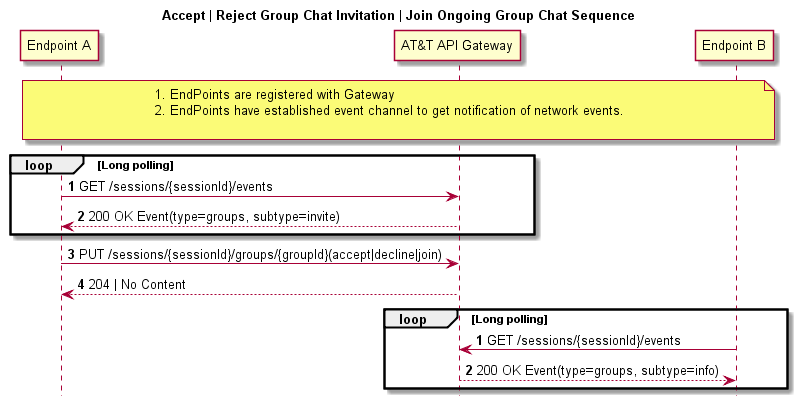
\includegraphics[width=0.6\paperwidth,height=0.4\paperheight]{sequence-diagram/AcceptRejectJoinGroup}

\pagebreak{}


\subsubsection{Version Impact Summary}

\begin{comment}
Summarize the different versions of this operation that are in production
or deleted by the current release of this service. 
\end{comment}


{\footnotesize{\begin{longtable}{|>{\raggedright}p{0.15\textwidth}|>{\raggedright}p{0.16\textwidth}|>{\raggedright}p{0.55\textwidth}|}
\hline
\hline 
\textbf{\footnotesize{Service Version}} & \textbf{\footnotesize{Major or Minor Impact}} & \textbf{\footnotesize{Changes Introduced by this Version}}\tabularnewline
\hline 
\hline
\endfirsthead
\hline
\hline 
\textbf{\footnotesize{Service Version}} & \textbf{\footnotesize{Major or Minor Impact}} & \textbf{\footnotesize{Changes Introduced by this Version}}\tabularnewline
\hline 
\hline
\endhead
\hline 
{\footnotesize{1}} & {\footnotesize{Major}} & {\footnotesize{Initial Release}}\tabularnewline
\hline 
\end{longtable}
}}{\footnotesize \par}


\subsubsection{Authentication and Authorization}

\begin{comment}
Describe OAuth model applicable to this operation.
\end{comment}


{\footnotesize{\begin{comment}
Describe OAuth model applicable to this operation.
\end{comment}


\begin{longtable}{|>{\raggedright}p{0.18\textwidth}|>{\raggedright}p{0.1\textwidth}|>{\raggedright}p{0.14\textwidth}|>{\raggedright}p{0.44\textwidth}|}
\hline
\hline 
\textbf{\footnotesize{Authorization Model}} & \textbf{\footnotesize{Subscriber Authorization required?}} & \textbf{\footnotesize{OAuth Scope Value}} & \textbf{\footnotesize{Brief Description}}\tabularnewline
\hline 
\hline
\endfirsthead
\hline
\hline 
\textbf{\footnotesize{Authorization Model}} & \textbf{\footnotesize{Subscriber Authorization required?}} & \textbf{\footnotesize{OAuth Scope Value}} & \textbf{\footnotesize{Brief Description}}\tabularnewline
\hline 
\hline
\endhead
\hline 
{\footnotesize{authorization\_code}} & {\footnotesize{Yes}} & {\footnotesize{RTC}} & \begin{enumerate}
\item {\footnotesize{Obtain the authorization code by passing App Key and
App Secret along with scope. This redirects the user to AT\&T authorization
page to capture user consent.}}{\footnotesize \par}
\item {\footnotesize{Obtain OAuth access token using the OAuth authorization
code along with the App Key and App Secret by making a Get Access
Token request with grant\_type=authorization\_code.}}{\footnotesize \par}

\begin{itemize}
\item {\footnotesize{Supports ICMN case}}\end{itemize}
\end{enumerate}
\tabularnewline
\hline 
{\footnotesize{client\_credentials}} & {\footnotesize{No}} & {\footnotesize{RTC}} & \begin{enumerate}
\item {\footnotesize{Obtain OAuth access token with the App Key and App
Secret along with the scope by making a Get Access Token request with
grant\_type=client\_credentials}}{\footnotesize \par}

\begin{itemize}
\item {\footnotesize{Supports VTN case }}{\footnotesize \par}
\item {\footnotesize{Supports no-TN case }}\end{itemize}
\end{enumerate}
\tabularnewline
\hline 
\end{longtable}
}}{\footnotesize \par}


\subsubsection{Representation Formats}

\begin{comment}
In the table below, describe supported representation formats for
the request and response body. Where different versions support different
formats, provide separate tables and indicate which versions apply
to each table. 
\end{comment}


{\footnotesize{
\subsubsection{Representation Formats}

\begin{comment}
In the table below, describe supported representation formats for
the request and response body. Where different versions support different
formats, provide separate tables and indicate which versions apply
to each table. 
\end{comment}


\begin{longtable}{|>{\raggedright}p{0.16\textwidth}|>{\raggedright}p{0.7\textwidth}|}
\hline
\hline 
\textbf{\footnotesize{Direction}} & \textbf{\footnotesize{Supported Respresentation Formats}}\tabularnewline
\hline 
\hline
\endfirsthead
\hline
\hline 
\textbf{\footnotesize{Direction}} & \textbf{\footnotesize{Supported Respresentation Formats}}\tabularnewline
\hline 
\hline
\endhead
\hline 
{\footnotesize{Request}} & {\footnotesize{XML, JSON,URLENCODED}}\tabularnewline
\hline 
{\footnotesize{Response}} & {\footnotesize{XML, JSON,URLENCODED}}\tabularnewline
\hline 
\end{longtable}
}}{\footnotesize \par}






\subsubsection{Input Parameters}

\begin{comment}
In the table below, describe input parameters. Where different versions
support different input parameters, provide separate tables and indicate
which versions apply to each table. The allowed values for the Location
in Request column are: Header, Resource URI, Body or Query Parameter.
\end{comment}


{\footnotesize{\begin{longtable}{|>{\raggedright}p{0.23\textwidth}|>{\raggedright}p{0.08\textwidth}|>{\raggedright}p{0.1\textwidth}|>{\raggedright}p{0.36\textwidth}|>{\raggedright}p{0.1\textwidth}|}
\hline
\hline 
\textbf{\footnotesize{Parameter }} & \textbf{\footnotesize{Data Type}} & \textbf{\footnotesize{Req?}} & \textbf{\footnotesize{Brief description}} & \textbf{\footnotesize{Location}}\tabularnewline
\hline 
\hline
\endfirsthead
\hline
\hline 
\textbf{\footnotesize{Parameter }} & \textbf{\footnotesize{Data Type}} & \textbf{\footnotesize{Req?}} & \textbf{\footnotesize{Brief description}} & \textbf{\footnotesize{Location}}\tabularnewline
\hline 
\hline
\endhead
\hline 
{\footnotesize{accept}} & {\footnotesize{String}} & {\footnotesize{No}} & {\footnotesize{Specifies the format of the body of the response. The
acceptable values for this parameter are:}}{\footnotesize \par}
\begin{itemize}
\item {\footnotesize{application/json}}{\footnotesize \par}
\item {\footnotesize{application/xml}}{\footnotesize \par}
\item {\footnotesize{application/x-www-form-urlencoded}}{\footnotesize \par}
\end{itemize}
{\footnotesize{The default value is application/json. }}{\footnotesize \par}

{\footnotesize{Per rfc2616: \textquotedbl{}If no Accept header field
is present, then it is assumed that the client accepts all media types.\textquotedbl{}
By default our services return application/json.}}{\footnotesize \par}

{\footnotesize{The normal Accept header processing rules shall be
followed according to rfc2616.}}{\footnotesize \par}

\emph{\footnotesize{Note}}{\footnotesize{: If there is no entity body
in a normal successful response, this parameter is still needed to
specify the format in the case of an error response message.}} & {\footnotesize{Header}}\tabularnewline
\hline 
{\footnotesize{authorization}} & {\footnotesize{String}} & {\footnotesize{Yes}} & {\footnotesize{Specifies the authorization type and token. The acceptable
format for this parameter is the phrase \textquotedbl{}Bearer OAuth
Token\textquotedbl{} followed by a space ( ) and an OAuth access token.
If this parameter value is missing from the header, then the API Gateway
returns a message with an HTTP status code of 400 Invalid Request.
If the OAuth access token is not valid, then the API Gateway returns
an HTTP status code of 401 Unauthorized with a WWW-Authenticate HTTP
header.}} & {\footnotesize{Header}}\tabularnewline
\hline 
{\footnotesize{content-length}} & {\footnotesize{Integer}} & {\footnotesize{No}} & {\footnotesize{Specifies the length of the content in octets. This
parameter is only required for a non-streaming request.}} & {\footnotesize{Header}}\tabularnewline
\hline 
{\footnotesize{content-type}} & {\footnotesize{String}} & {\footnotesize{Yes}} & {\footnotesize{Specifies the type of content of the body. The acceptable
values for this parameter are:}}{\footnotesize \par}
\begin{itemize}
\item {\footnotesize{application/xml}}{\footnotesize \par}
\item {\footnotesize{application/json}}\end{itemize}
 & {\footnotesize{Header}}\tabularnewline
\hline 
{\footnotesize{transfer-encoding}} & {\footnotesize{String}} & {\footnotesize{Conditional}} & {\footnotesize{Specifies the encodingof the message. The only acceptable
values for this parameter is:}}{\footnotesize \par}
\begin{itemize}
\item {\footnotesize{chunked}}{\footnotesize \par}
\end{itemize}
{\footnotesize{This parameter is only required for a streaming request.}} & {\footnotesize{Header}}\tabularnewline
\hline 
{\footnotesize{x-invitation}} & {\footnotesize{String}} & {\footnotesize{Yes}} & {\footnotesize{Specifies the answer to the invitation. The acceptable
values for this parameter are:}}{\footnotesize \par}
\begin{itemize}
\item {\footnotesize{accept : The participant accepts the chat invitation.}}{\footnotesize \par}
\item {\footnotesize{decline : The participant rejects the chat invitation.}}{\footnotesize \par}
\item {\footnotesize{join : Th participant joins ongoing group chat conversation.}}\end{itemize}
 & {\footnotesize{Header}}\tabularnewline
\hline 
\end{longtable}



{\footnotesize{}}
}}{\footnotesize \par}


\paragraph{Request – Example (Accept invitation to join a chat group - XML)\protect \\
}



This demostrates how to accept invitation to join a group using xml.

\begin{lstlisting}[backgroundcolor={\color{shadebox}},basicstyle={\footnotesize\ttfamily},frame=single,framerule={.5pt}]
PUT  /RTC/v1/sessions/4ba569b5-290d-4f1f-b3af-255731383204/groups/j7q5bL HTTP/1.1 
Host: api.att.com
authorization: Bearer abcdef12345678
accept: application/xml
content-type: application/xml
x-invitation: accept
\end{lstlisting}



\paragraph{Request – Example (Accept invitation to join a chat group - JSON)\protect \\
}

This demostrates how to accept invitation to join a group using JSON.

\begin{lstlisting}[backgroundcolor={\color{shadebox}},basicstyle={\footnotesize\ttfamily},frame=single,framerule={.5pt}]
PUT  /RTC/v1/sessions/4ba569b5-290d-4f1f-b3af-255731383204/groups/j7q5bL HTTP/1.1
Host: api.att.com
authorization: Bearer 38C2399A23999 
accept: application/json
content-length: 300
content-type: application/json
x-invitation: accept
\end{lstlisting}



\paragraph{Request – Example (Reject invitation to join a chat group - XML)}

This demostrates how to accept invitation to join a group using xml.

\begin{lstlisting}[backgroundcolor={\color{shadebox}},basicstyle={\footnotesize\ttfamily},frame=single,framerule={.5pt}]
PUT  /RTC/v1/sessions/4ba569b5-290d-4f1f-b3af-255731383204/groups/j7q5bL HTTP/1.1 
Host: api.att.com
authorization: Bearer abcdef12345678
accept: application/xml
content-type: application/xml
x-invitation: decline
\end{lstlisting}



\paragraph{Request – Example (Reject invitation to join a chat group- JSON)}

This demostrates how to reject invitation to join a group using JSON.

\begin{lstlisting}[backgroundcolor={\color{shadebox}},basicstyle={\footnotesize\ttfamily},frame=single,framerule={.5pt}]
PUT  /RTC/v1/sessions/4ba569b5-290d-4f1f-b3af-255731383204/groups/j7q5bL HTTP/1.1
Host: api.att.com
authorization: Bearer 38C2399A23999 
accept: application/json
content-length: 300
x-invitation: decline
\end{lstlisting}



\paragraph{Request – Example (Join ongoing chat conversation - JSON)}

This demostrates how to reject invitation to join a group using JSON.

\begin{lstlisting}[backgroundcolor={\color{shadebox}},basicstyle={\footnotesize\ttfamily},frame=single,framerule={.5pt}]
PUT /RTC/v1/sessions/4ba569b5-290d-4f1f-b3af-255731383204/chatGroups/j7q5bL HTTP/1.1
Host: api.att.com
authorization: Bearer 38C2399A23999 
accept: application/json
content-length: 300
content-type: application/json
x-invitation: join
\end{lstlisting}



\subsubsection{Output Parameters}

\begin{comment}
In the table below, describe output parameters. Where different versions
support different output parameters, provide separate tables and indicate
which versions apply to each table. Note: ‘consent’ refers to end
user consent which may need to be obtained before data is returned,
\end{comment}


{\footnotesize{{\footnotesize{}}%
\begin{longtable}{|>{\raggedright}p{0.23\textwidth}|>{\raggedright}p{0.08\textwidth}|>{\raggedright}p{0.05\textwidth}|>{\raggedright}p{0.41\textwidth}|>{\raggedright}p{0.1\textwidth}|}
\hline
\hline 
\textbf{\footnotesize{Parameter }} & \textbf{\footnotesize{Data Type}} & \textbf{\footnotesize{Req?}} & \textbf{\footnotesize{Brief description}} & \textbf{\footnotesize{Location}}\tabularnewline
\hline 
\hline
\endfirsthead
\hline
\hline 
\textbf{\footnotesize{Parameter }} & \textbf{\footnotesize{Data Type}} & \textbf{\footnotesize{Req?}} & \textbf{\footnotesize{Brief description}} & \textbf{\footnotesize{Location}}\tabularnewline
\hline 
\hline
\endhead
\hline 
{\footnotesize{content-type}} & {\footnotesize{String}} & {\footnotesize{Yes}} & {\footnotesize{Specifies the type of content of the body. The acceptable
values for this parameter are:}}{\footnotesize \par}
\begin{itemize}
\item {\footnotesize{application/xml}}{\footnotesize \par}
\item {\footnotesize{application/json}}\end{itemize}
 & {\footnotesize{Header}}\tabularnewline
\hline 
\end{longtable}{\footnotesize \par}

{\footnotesize{}}
}}{\footnotesize \par}


\paragraph{Response – Example (Accept invitation to join a chat group - XML)\protect \\
}

This shows the response to a accept/reject invitation to join a chat
group XML format.

\texttt{}
\begin{lstlisting}[basicstyle={\footnotesize\ttfamily},tabsize=4]
HTTP/1.1 204 No Content
Content-Type: application/xml 
Content-Length: 100 
Date: Tue, 04 Dec 2013 02:51:59 GMT
\end{lstlisting}



\paragraph{Response – Example (Joining ongoing group conversation - XML)\protect \\
}

This shows the response to joining ongoing group conversation XML
format.

\texttt{}
\begin{lstlisting}[basicstyle={\footnotesize\ttfamily},tabsize=4]
HTTP/1.1 202 Accepted
Content-Type: application/xml 
Content-Length: 100 
Date: Tue, 04 Dec 2013 02:51:59 GMT
\end{lstlisting}



\subsubsection{Service Exceptions}

\begin{comment}
List the service exceptions generated by the operation (indicate any
variation that exists across different versions):
\end{comment}


\begin{longtable}{|>{\raggedright}p{0.1\textwidth}|>{\raggedright}p{0.33\textwidth}|>{\raggedright}p{0.33\textwidth}|>{\raggedright}p{0.1\textwidth}|}
\hline
\hline 
\textbf{\footnotesize{MessageId}} & \textbf{\footnotesize{Text}} & \textbf{\footnotesize{Variables}} & \textbf{\footnotesize{Parent HTTP Code}}\tabularnewline
\hline 
\hline
\endfirsthead
\hline
\hline 
\textbf{\footnotesize{MessageId}} & \textbf{\footnotesize{Text}} & \textbf{\footnotesize{Variables}} & \textbf{\footnotesize{Parent HTTP Code}}\tabularnewline
\hline 
\hline
\endhead
\hline 
{\footnotesize{SVC0001}} & {\footnotesize{A service error has occurred. Error code is <error\_explanation>}} & {\footnotesize{error\_explanation : <content\_here>}} & {\footnotesize{400}}\tabularnewline
\hline 
{\footnotesize{SVC0002}} & {\footnotesize{Invalid input value for Message part <part\_name>}} & {\footnotesize{part\_name : name of the input parameter that resulted
in the error.}} & {\footnotesize{400}}\tabularnewline
\hline 
{\footnotesize{SVC0003}} & {\footnotesize{Invalid input value for Message part <part\_name>,
valid values are <part\_values>}} & {\footnotesize{part\_name : name of the input parameter that resulted
in the error.}}{\footnotesize \par}

{\footnotesize{part\_value : value of input parameter that was found
to be in error.}} & {\footnotesize{400}}\tabularnewline
\hline 
{\footnotesize{SVC0004}} & {\footnotesize{No valid addresses provided in the Message part <part\_name>}} & {\footnotesize{part\_name : name of the input parameter that resulted
in the error.}} & {\footnotesize{400}}\tabularnewline
\hline 
\end{longtable}


\subsubsection{Policy Exceptions}

\begin{comment}
List the policy exceptions generated by the operation (indicate any
variation that exists across different versions):
\end{comment}


\begin{longtable}{|>{\raggedright}p{0.1\textwidth}|>{\raggedright}p{0.33\textwidth}|>{\raggedright}p{0.33\textwidth}|>{\raggedright}p{0.1\textwidth}|}
\hline
\hline 
\textbf{\footnotesize{MessageId}} & \textbf{\footnotesize{Text}} & \textbf{\footnotesize{Variables}} & \textbf{\footnotesize{Parent HTTP Code}}\tabularnewline
\hline 
\hline
\endfirsthead
\hline
\hline 
\textbf{\footnotesize{MessageId}} & \textbf{\footnotesize{Text}} & \textbf{\footnotesize{Variables}} & \textbf{\footnotesize{Parent HTTP Code}}\tabularnewline
\hline 
\hline
\endhead
\hline 
{\footnotesize{POL0001}} & {\footnotesize{A policy error occurred. For example, rate limit error,
authentication and authorization error.}} & {\footnotesize{N/A}} & {\footnotesize{401, 403}}\tabularnewline
\hline 
{\footnotesize{POL0002}} & {\footnotesize{Privacy verification failed for address <address>,
request is refused}} & {\footnotesize{address : <content\_here>}} & {\footnotesize{403}}\tabularnewline
\hline 
{\footnotesize{POL0003}} & {\footnotesize{Too many addresses specified in Message part}} & {\footnotesize{N/A}} & {\footnotesize{403}}\tabularnewline
\hline 
{\footnotesize{POL1009}} & {\footnotesize{User has not been provisioned for \%1}} & {\footnotesize{1\% : System that has not been provisioned}} & {\footnotesize{403}}\tabularnewline
\hline 
\end{longtable}

\end{document}
